\section{\Acrfull{bsj} detection}

For detection of \gls{bsj}s, I used the five tools already introduced in
\cref{subsec:circrna_detection}.
As shown in \cref{fig:detection_bars}, find\_circ, CIRI2, DCC, and
circexplorer2 detect a similar number of \gls{bsj}s, while segemehl detects
almost ten times as many \gls{bsj}s as its closest competitor, DCC.

\begin{figure}[ht] \centering

    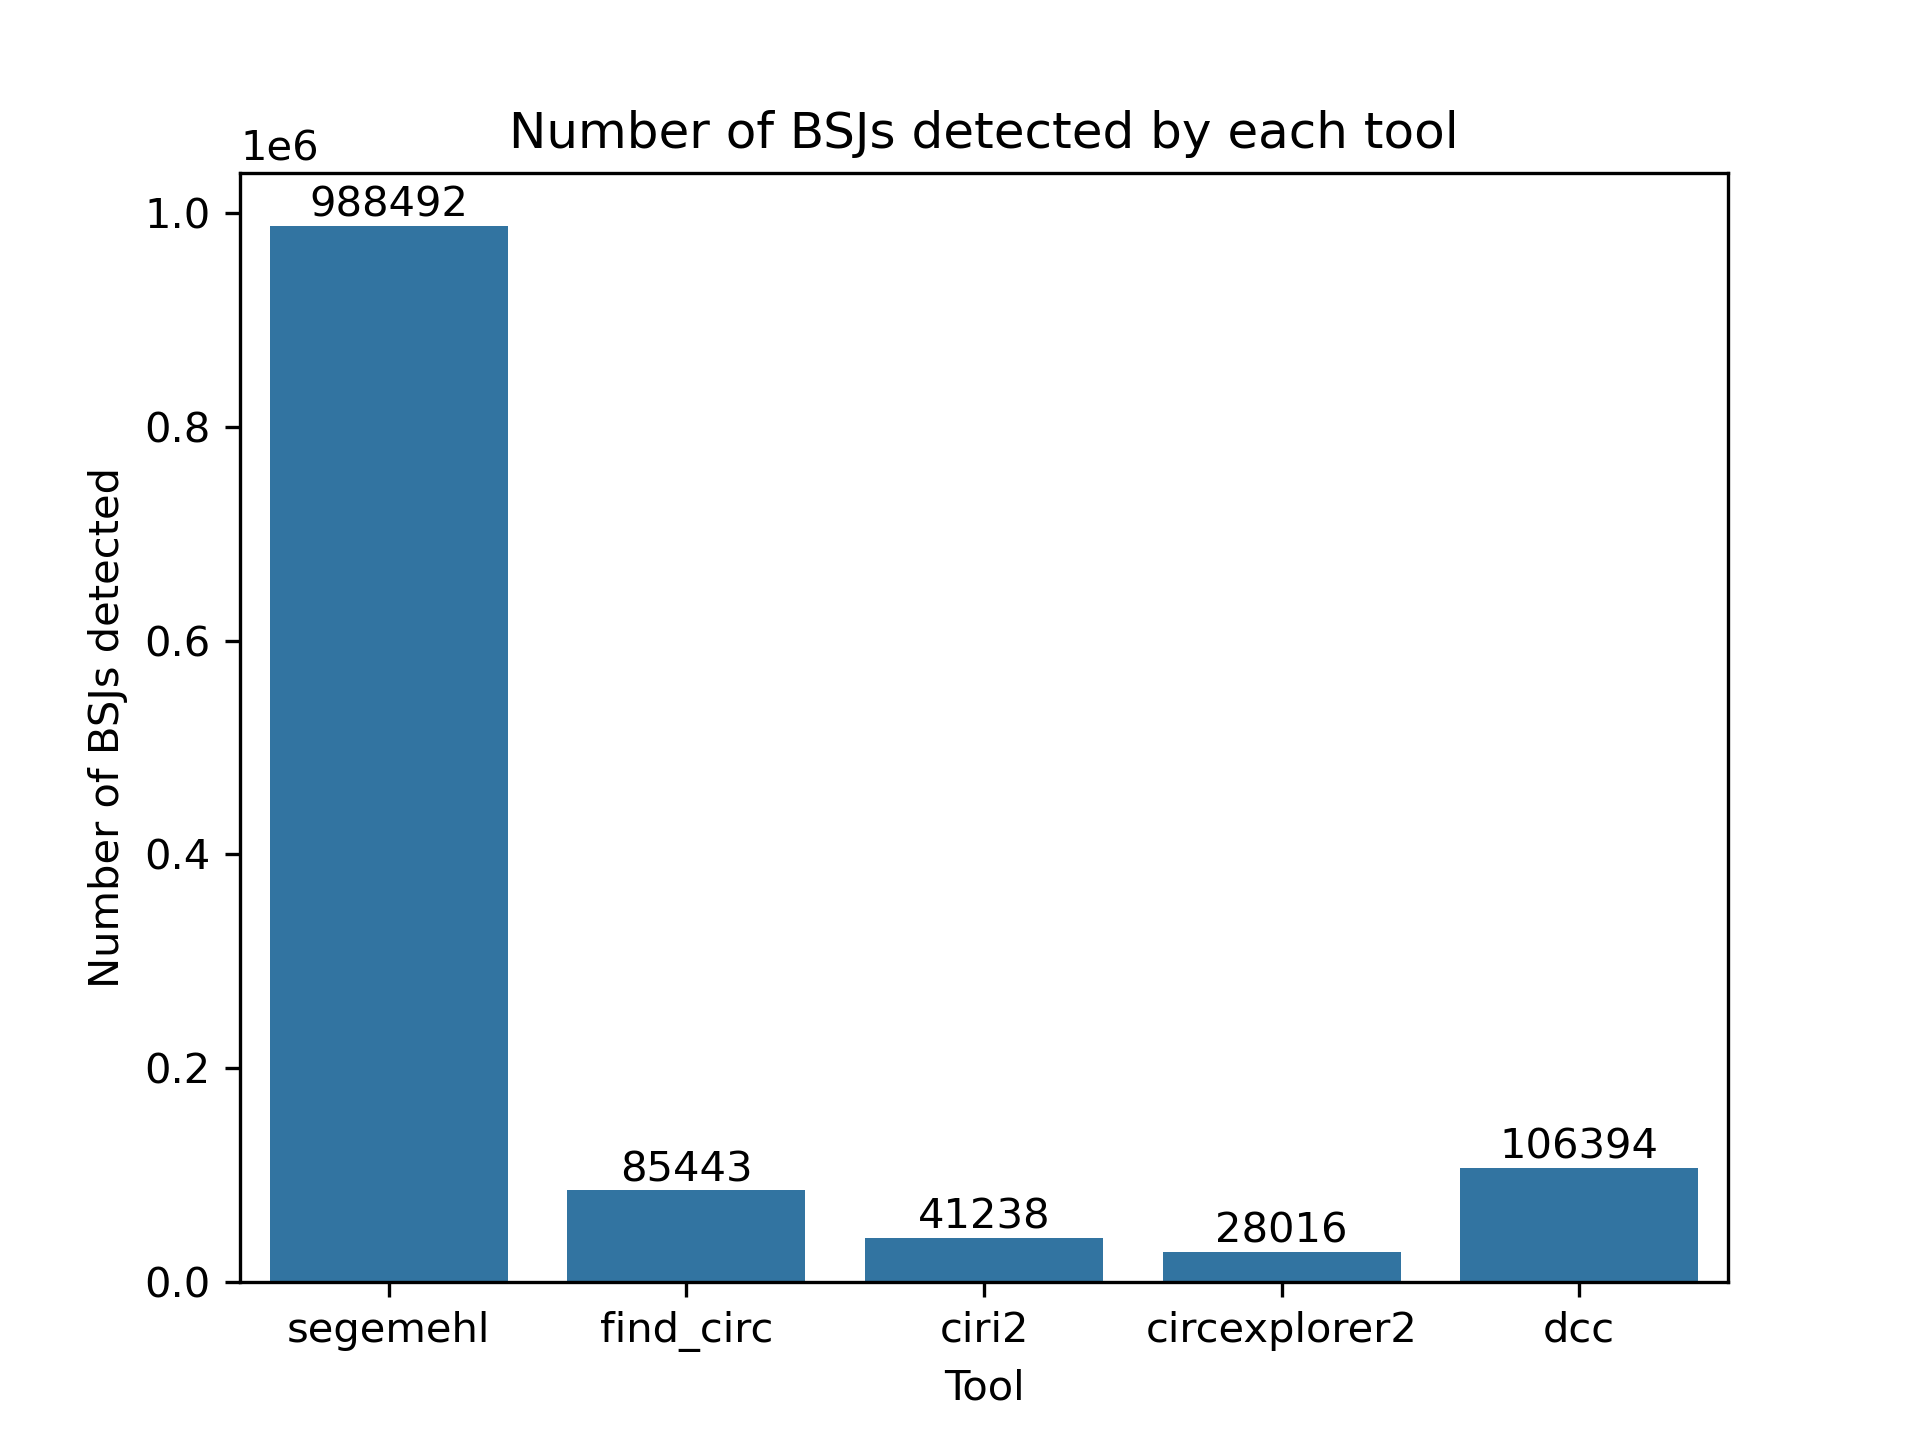
\includegraphics[width=0.6\textwidth]{chapters/4_results_and_discussion/figures/detection/n_bsjs_detected.png}
    \caption{Number of \gls{bsj}s detected by each tool.
        While find\_circ, CIRI2, DCC and circexplorer2 detect a similar number of
        \gls{bsj}s, segemehl detects a much larger number of \gls{bsj}s.
    }
    \label{fig:detection_bars}
\end{figure}
Similar behavior was previously observed by \textcite{zeng_comprehensive_2017},
where segemehl was among the top performers in terms of sensitivity, but also
had a high false positive rate.
The lowest numbers of \gls{bsj}s were detected by circexplorer2 and CIRI2,
which both have built-in filters to reduce false
positives\supercite{zhang_diverse_2016,gao_circular_2018}.

\subsection{Agreement between tools and the role of \textit{max shift}}

Although tools like CIRI2 and CircExplorer2 have shown good performance in
benchmarks, having multiple tools agree on the same \gls{bsj} can be a good
indicator of the reliability of the detection.

To assess the agreement between the tools, I used UpSet plots, which show the
overlap of \gls{bsj}s detected by different tools.
When identifying the overlap between tools, the most strict approach is to
consider only \gls{bsj}s with identical start and end positions and on the same
strand as the same \gls{bsj}.
The according plot is shown in \cref{fig:detection_upset_0}.
While there are a total of x \gls{bsj}s detected by at least two tools, only y
\gls{bsj}s are detected by three tools, and none are detected by four or five
tools.

\begin{figure}[ht]
    \centering

    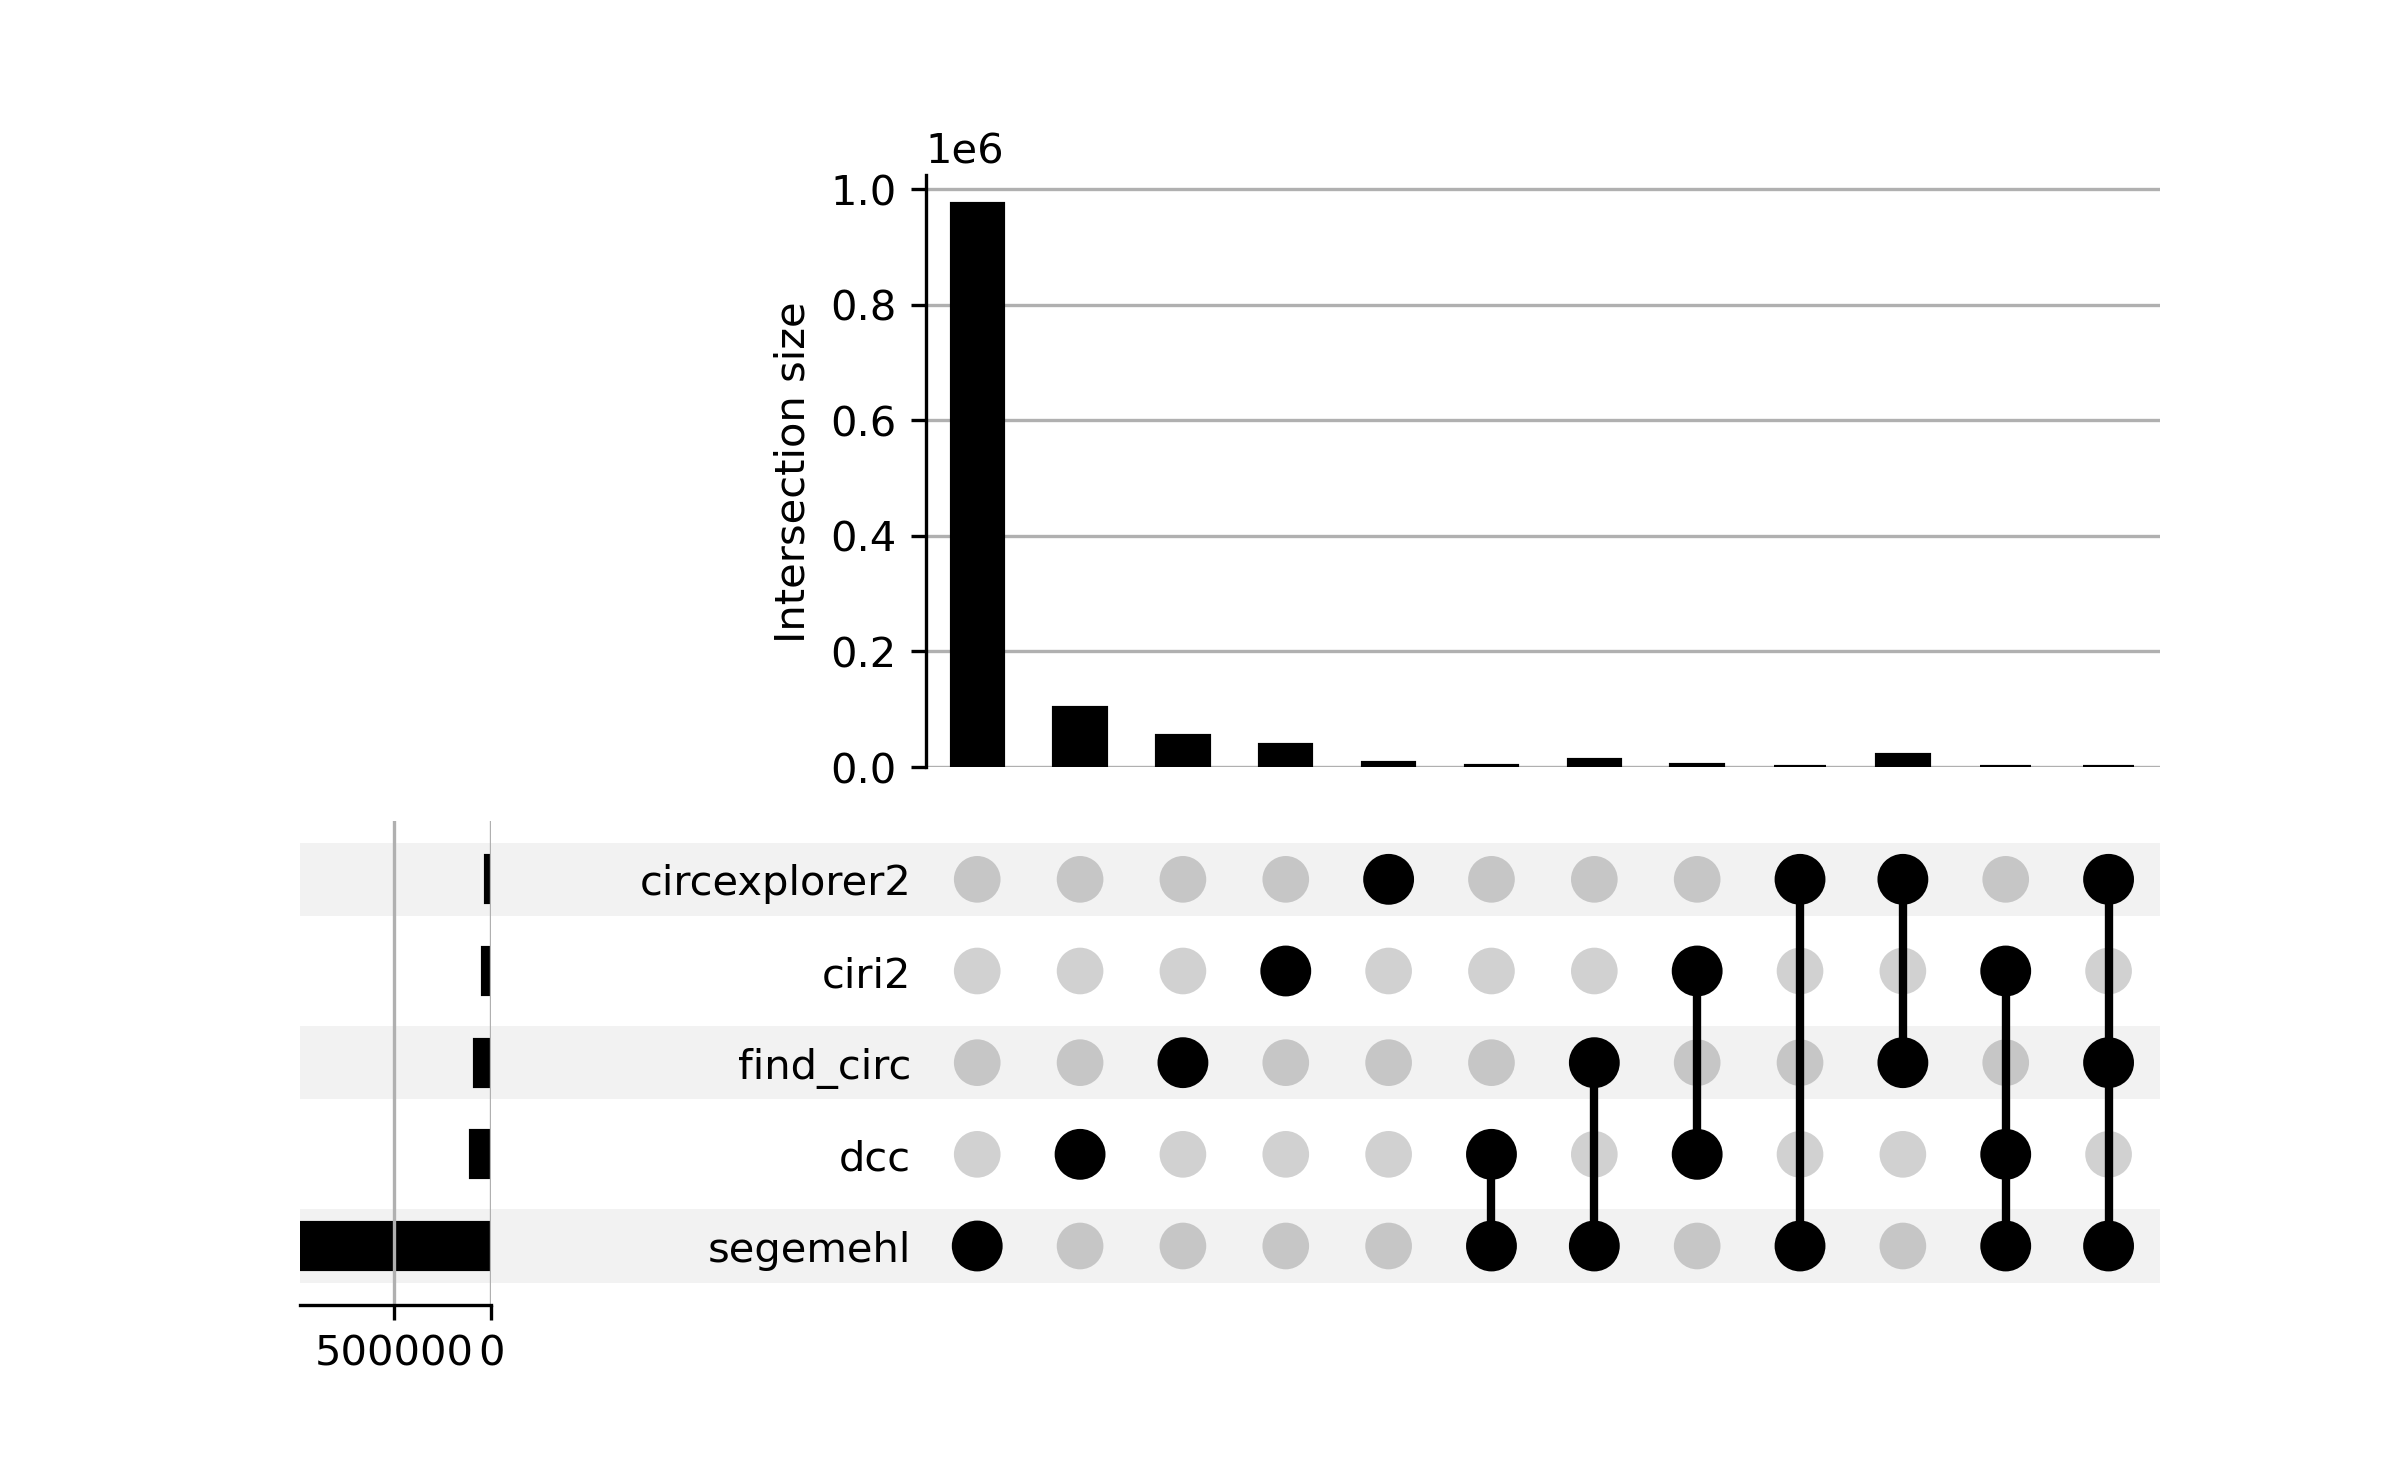
\includegraphics[width=\textwidth]{chapters/4_results_and_discussion/figures/detection/upset/shift_0.png}
    \caption{Upset plot illustrating the overlap between \gls{bsj}s detected by
        different tools.
        Only \gls{bsj}s with identical start and end positions are considered the same.
        Only combinations with at least 10 common \gls{bsj}s are shown.
    }
    \label{fig:detection_upset_0}
\end{figure}

As this agreement is relatively low, I investigated the detected \gls{bsj}s
more closely and found that tools often have very similar \gls{bsj}s, but with
slight differences in the start and end positions.

In order to quantify how frequently the slight mismatches occur, I introduced a
\textit{max shift} parameter.
With this parameter, if tool A detects a \gls{bsj} and tool B detects another
\gls{bsj}, where the start and end positions differ by at most \textit{max
    shift} nucleotides, both \gls{bsj}s are considered to be supported by both
tools.
A more detailed explanation is given in \cref{fig:detection_shift_schematic}.

\begin{figure}[ht] \centering

    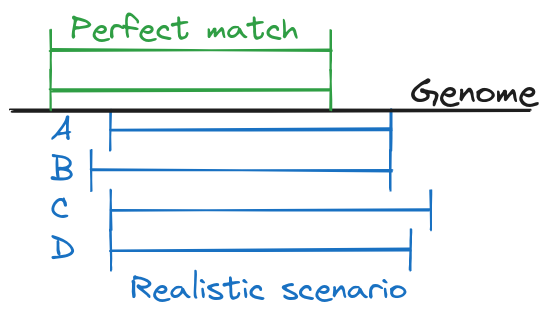
\includegraphics[width=0.7\textwidth]{chapters/4_results_and_discussion/figures/grouping.png}
    \caption{Schematic illustrating two different scenarios of \gls{bsj}
        matches
        across tools.
        In the green scenario, the \gls{bsj}s are exactly the same.
        This is what is required in order to be counted as a match in
        \cref{fig:detection_upset_0}.
        However, this rarely occurs in practice.
        More frequently, the scenario illustrated in blue occurs.
        Here, tools detect very similar \gls{bsj}s, with only a few nucleotides
        difference.
        In order to account for this, a \textit{max shift} parameter is introduced.
        While in the blue scenario, all \gls{bsj}s would only be supported by one tool,
        with a \textit{max shift} of 1, the result would change drastically.
        The \gls{bsj} marked as A would be supported by two others (B and D), similarly
        B would be supported by two others (A and D).
        C would only be supported by D, as both the ends of both A and B differ by more
        than 1.
        D would be supported by all others.
    }
    \label{fig:detection_shift_schematic}
\end{figure}

In order to quantify the magnitude of the effect of the \textit{max shift}
parameter, I calculated the level of agreement between tools for different
values of \textit{max shift}.
The results are shown in \cref{fig:shift_agreement}.

\begin{figure}[ht]
    \centering

    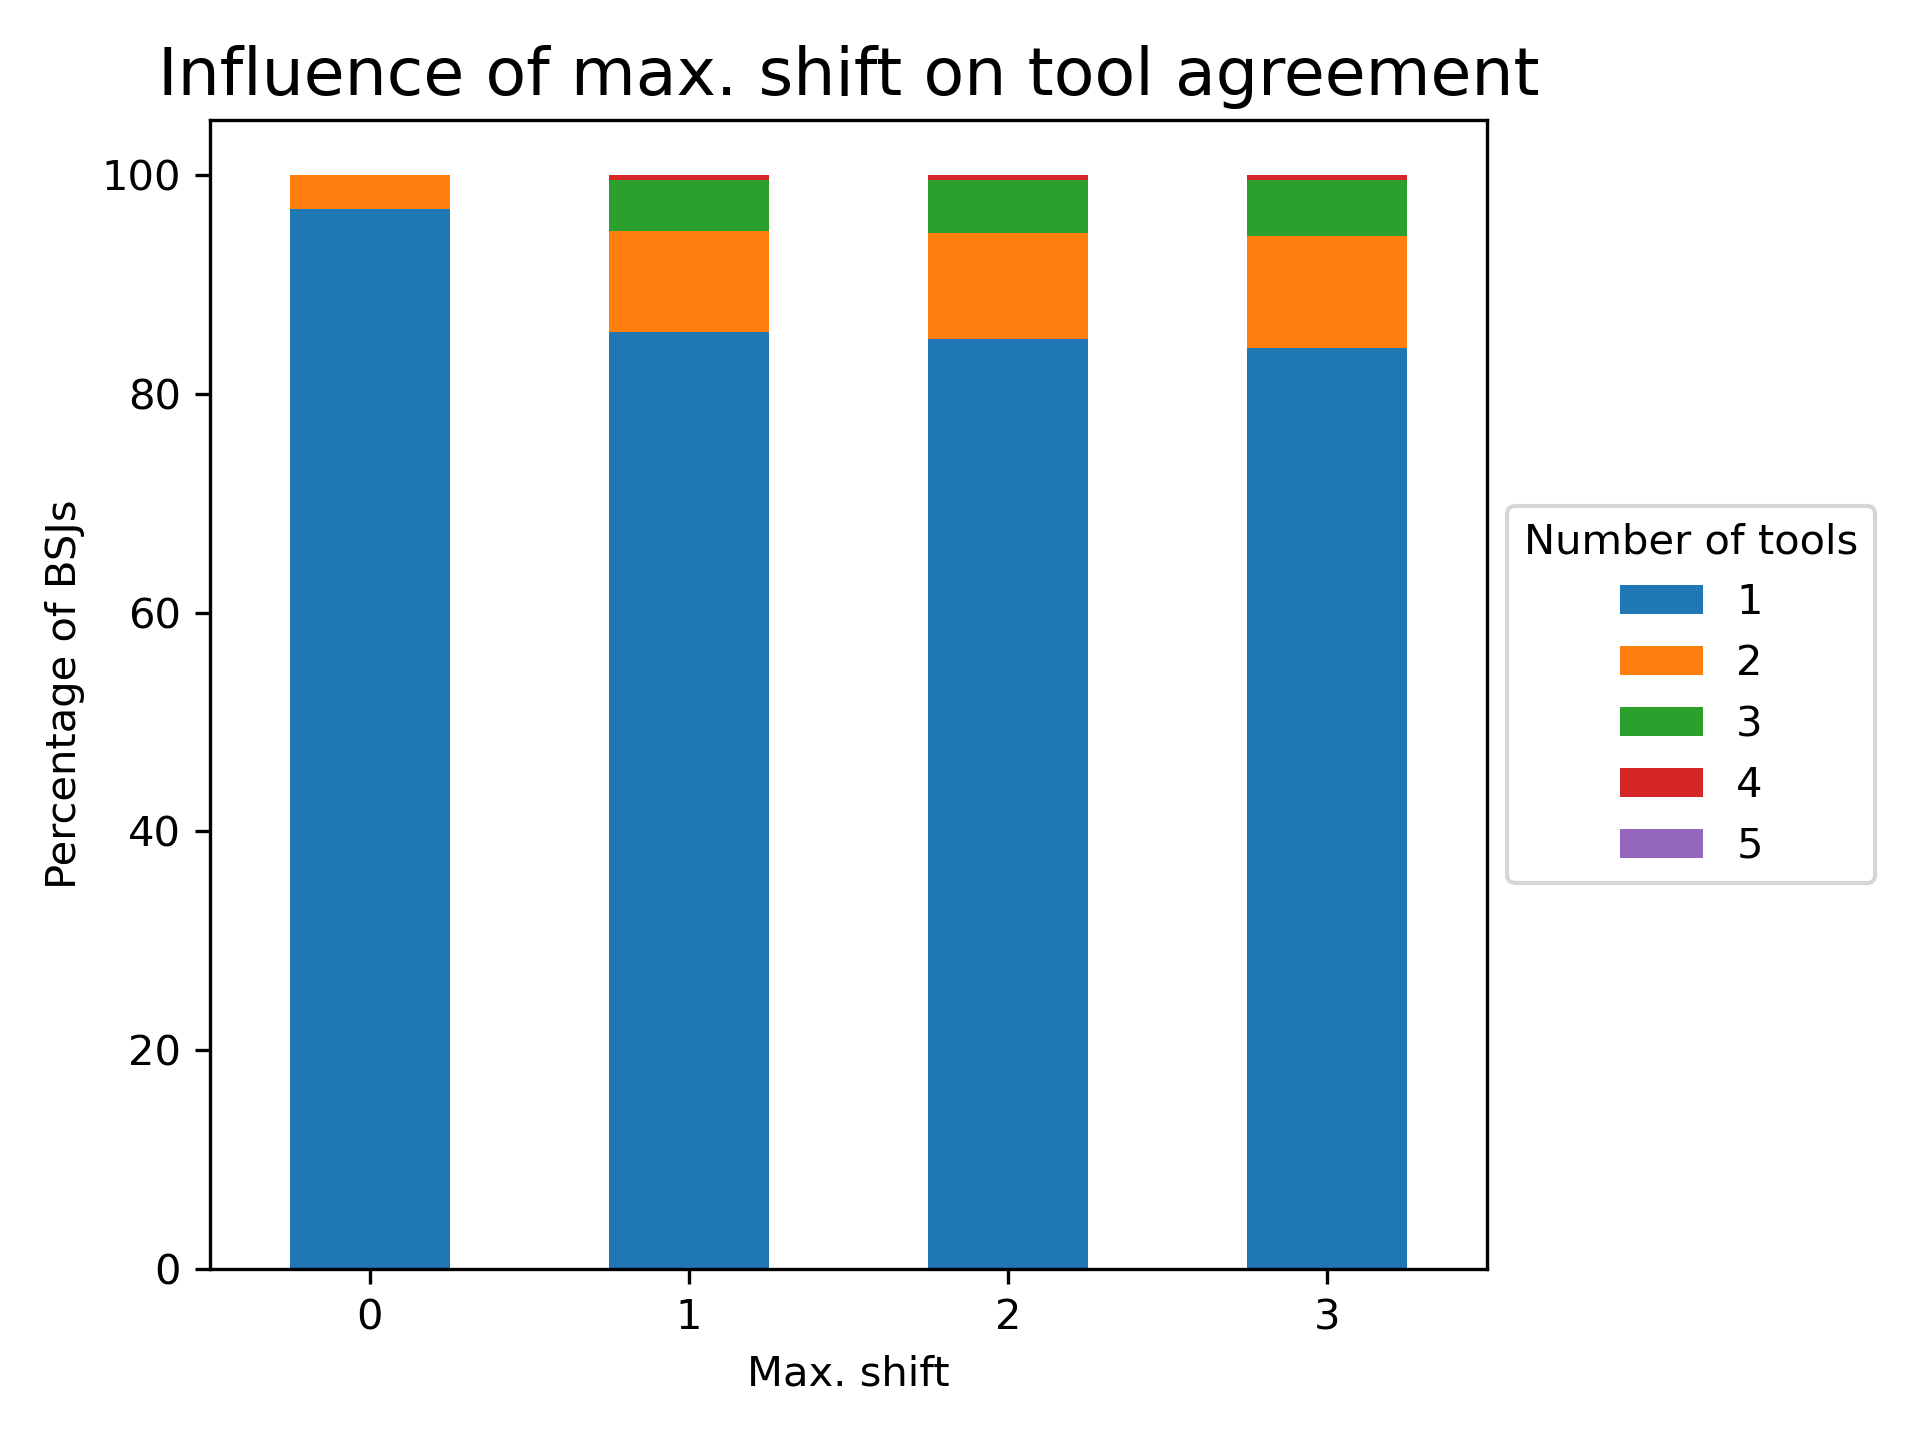
\includegraphics[width=0.7\textwidth]{chapters/4_results_and_discussion/figures/detection/shift_agreement.png}
    \caption{Stacked bar plot showing the level of agreement between tools for
        different values of the \textit{max shift} parameter.
        While the distribution changes drastically when increasing the \textit{max
            shift} parameter from 0 to 1, the distribution remains relatively stable for
        higher values.
        While the number of \gls{bsj}s detected by 2-3 tools continues to increase when
        raising the \textit{max shift} parameter to 20 or 50, the number of \gls{bsj}s
        detected by 4-5 tools remains nearly constant.
    }
    \label{fig:shift_agreement}
\end{figure}

As shown in \cref{fig:shift_agreement}, the distribution of the number of tools
supporting a \gls{bsj} changes drastically when increasing the \textit{max
    shift} parameter from 0 to 1.
However, the distribution remains relatively stable, especially for agreement
between four or five tools.
Increasing the \textit{max shift} parameter to large values does have an effect
on the number of \gls{bsj}s detected by two or three tools, but this comes with
the risk of increasing the number of false positives, since this way \gls{bsj}s
with a relatively large difference in start and end positions are still
considered as evidence for each other.

For the following analyses, I chose a \textit{max shift} parameter of 3 and a
minimum agreement of 4 tools, as this appeared to be a good compromise between
sensitivity and specificity.
The resulting UpSet plot is shown in \cref{fig:detection_upset_3}.

\begin{figure}[ht]
    \centering

    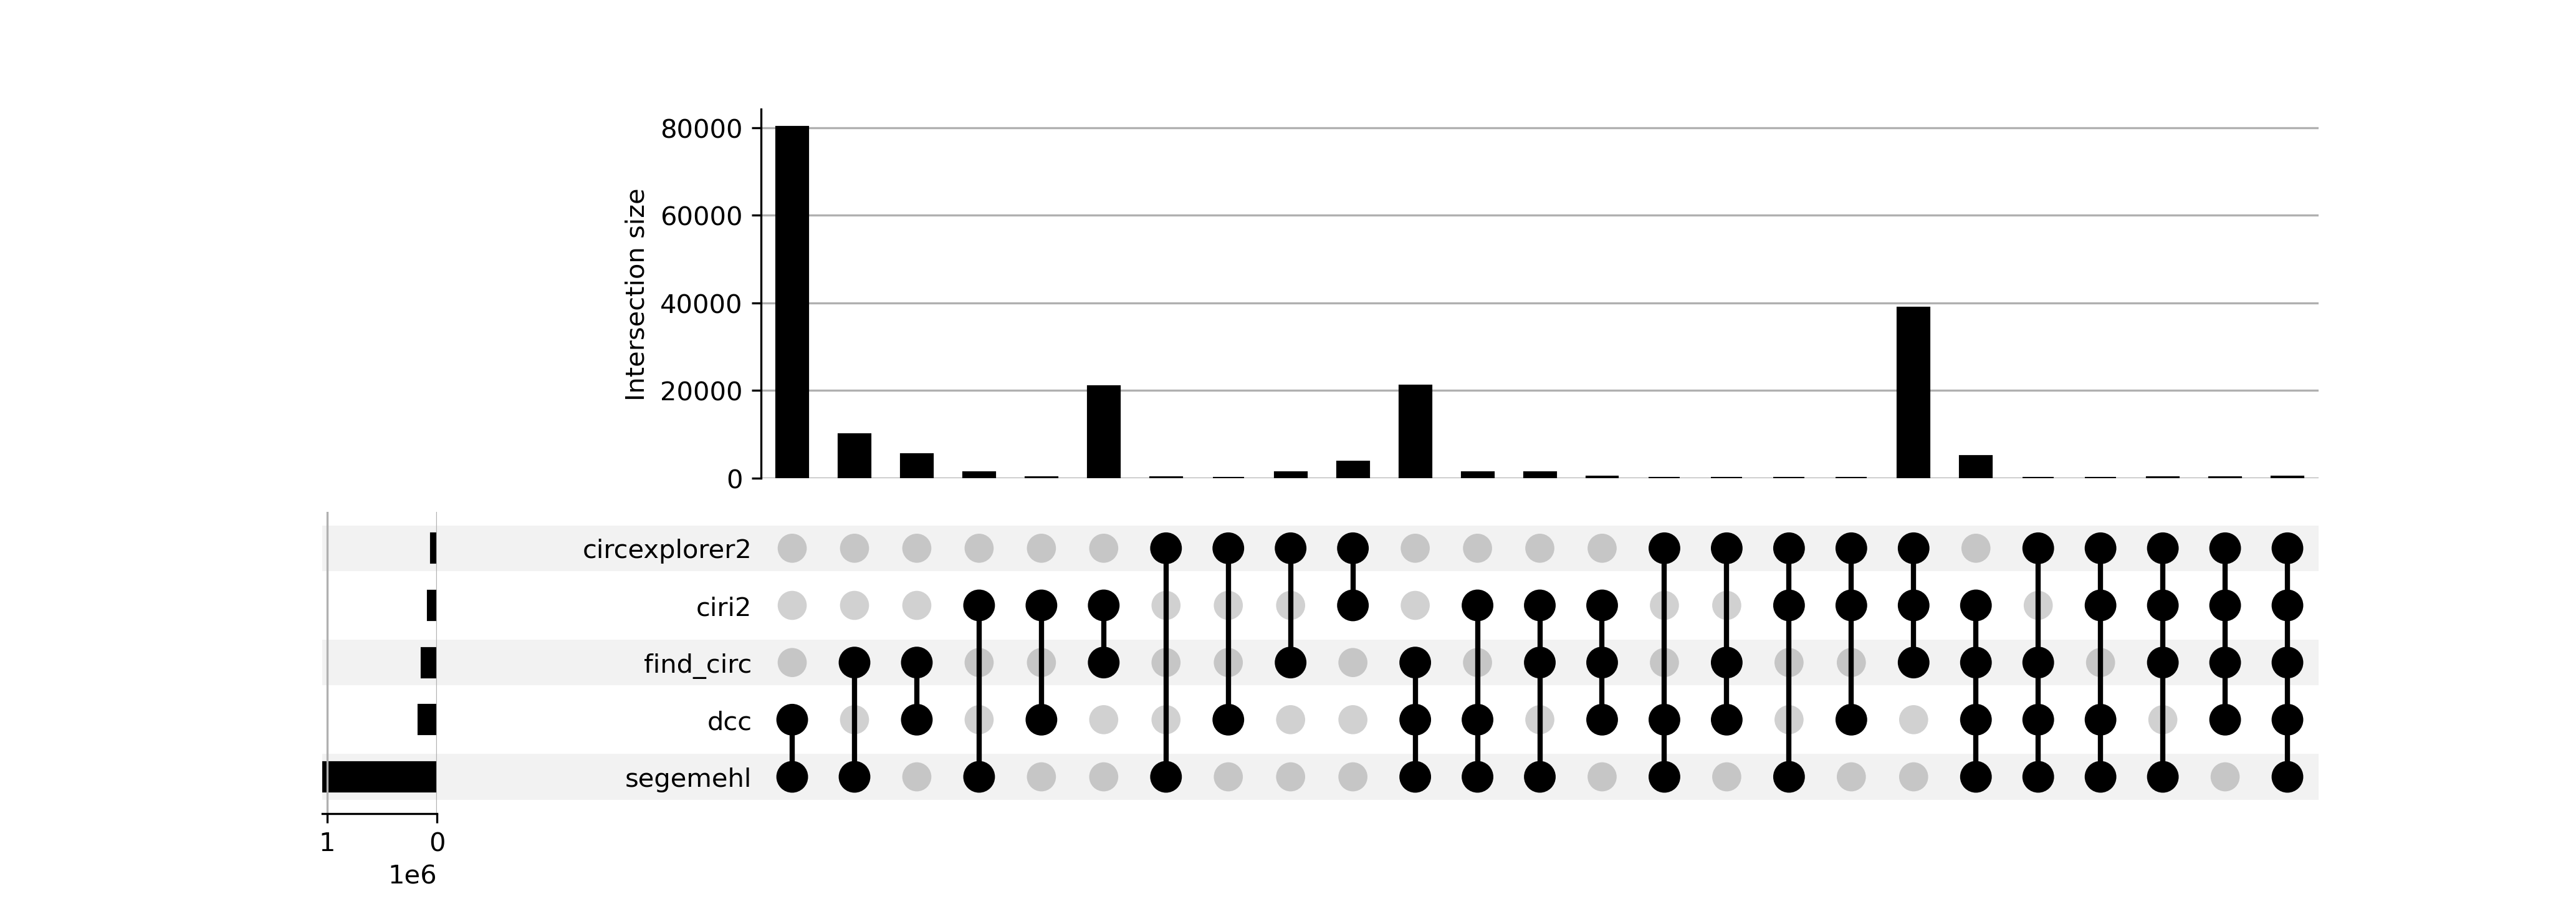
\includegraphics[width=\textwidth]{chapters/4_results_and_discussion/figures/detection/upset/shift_3.png}
    \caption{Upset plot illustrating the overlap between \gls{bsj}s detected by
        different tools.
        Agreement was calculated using a \textit{max shift} of 3.
        Only combinations including at least 2 tools and 10 common \gls{bsj}s are
        shown.
    }
    \label{fig:detection_upset_3}
\end{figure}
